% tri_monophase_transformer.tex
% Three-phase to single-phase transformer with two star-connected primaries on a three-limb
% core: magnetic model, steady-state behaviour and Simscape implementation
% (tri_monophase_transformer.ssc, pwr-control/library).
% pwr-control template (AAA_template_latex_settings); numbers and figures of Section 6:
% tri_monophase_transformer_check.py (python3, numpy + matplotlib)
% Compile: pdflatex tri_monophase_transformer.tex  (twice, for references)
% Rev. 00 - October 2026 - first issue
\documentclass[10pt,a4paper]{scrartcl}
% ===================== PACKAGES =====================
\usepackage[british]{babel}
\usepackage[tmargin=1in, bmargin=1in, lmargin=0.75in, rmargin=0.75in]{geometry}
\usepackage[dvipsnames,table]{xcolor}  % prima di tikz, listings, ecc.

\usepackage{tikz}
\usepackage{graphicx}
\usepackage{pgfplots}
\pgfplotsset{width=12cm, compat=1.9}
\usepackage{setspace}
\usepackage{chemmacros}
\usepackage{chemfig}
\usepackage{esint}
\usepackage{tabularray}
\usepackage{makeidx}
\usepackage{epstopdf}
\usepackage{amssymb}
\usepackage{mathrsfs}
\usepackage{bm}
\usepackage{amsmath}
\usepackage{enumitem}
\usepackage[english]{varioref}
\usepackage{lipsum}
\usepackage{fancyhdr}
\usepackage{float}
\usepackage{empheq}
\usepackage[framemethod=tikz]{mdframed}
\numberwithin{equation}{section}
\usepackage{eso-pic}
\usepackage{calc}
\usepackage{nccmath}
\usepackage{caption}
\usepackage{subcaption}
\usepackage{gensymb}
\usepackage{amsfonts, amsthm, epsfig, epstopdf, titling, url, array}
\usepackage{tabularx}
\usepackage{makecell}
\usepackage{booktabs}
\usepackage{array}
\usepackage{siunitx}
\sisetup{input-digits=0123456789\pi}
\usepackage[symbol]{footmisc}
\usepackage{multicol}
\usepackage{boondox-cal}
\usepackage{blindtext}
\usepackage{changepage}
\usepackage{nomencl}
\usepackage{hyperref}
\usepackage{xurl}
\usepackage{ragged2e}
\usepackage[version=4]{mhchem}  % ← conflitto di opzioni
\usepackage{longtable}
\usepackage{chemformula}
\usetikzlibrary{arrows.meta,positioning,calc}

% ===================== SI UNITS =====================
\DeclareSIUnit\atm{atm}
\DeclareSIUnit{\var}{var}
\DeclareSIUnit{\pu}{p.u.}


% ===================== MATH OPERATORS =====================
\DeclareMathOperator{\rank}{rank}
\DeclareMathOperator{\atantwo}{atan2}
\DeclareMathOperator{\spn}{span}

% ===================== COMMANDS =====================
\newcommand{\abs}[1]{\left|#1\right|}
\newcommand{\sign}{\text{sign}}
\newcommand{\centered}[1]{\begin{tabular}{@{}l@{}} #1 \end{tabular}}

% ===================== COLORS =====================
\definecolor{mycolor1}{rgb}{0.97, 0.97, 0.97}
\definecolor{mycolor2}{rgb}{0.97, 0.97, 0.97}
\definecolor{tableShade}{gray}{0.9}

% ===================== THEOREM ENVIRONMENTS =====================
\theoremstyle{it}
\newtheorem{defn}{Definition}[section]
\newtheorem{assumption}{Assumption}[section]
\newtheorem{thm}{Theorem}[section]
\newtheorem{lemma}{Lemma}[section]
\newtheorem{corollary}{Corollary}[section]
\theoremstyle{definition}
\newtheorem{example}{Example}[section]

% ===================== CUSTOM ENVIRONMENTS =====================
\newenvironment{myitemize_1}{
	\begin{itemize}[topsep=0pt]
		\setlength{\topsep}{2pt}
		\setlength{\itemsep}{2pt}
		\setlength{\parskip}{2pt}
		\setlength{\parsep}{2pt}
	}{\end{itemize}}

\newmdenv[
innerlinewidth=0.5pt,
roundcorner=4pt,
backgroundcolor=mycolor2,
linecolor=mycolor1,
innerleftmargin=6pt,
innerrightmargin=6pt,
innertopmargin=6pt,
innerbottommargin=6pt
]{mybox}

% ===================== TABLE COLUMN TYPES =====================
\newcolumntype{Y}{>{\hsize=2\hsize}X}
\newcolumntype{Z}{>{\centering\arraybackslash\hsize=0.857\hsize}X}

% ===================== SECTION DEPTH =====================
\setcounter{secnumdepth}{3}
\setcounter{tocdepth}{3}

% ===================== PAGE STYLE =====================
\setlength{\headheight}{20pt}
\setlength{\headsep}{20pt}

\pagestyle{fancy}
\fancypagestyle{firstpage}{\rhead{}}
\fancyhead[L]{\slshape\nouppercase{\leftmark}}
\chead{}
\rhead{\includegraphics[height=0.75cm]{../../AAA_template_latex_settings/pwr-control_logo_doc.png}}
\lfoot{\href{http://www.pwr-control.com}{pwr-control.com}}
\cfoot{-\ \thepage\ -}
\rfoot{\textit{}}
\renewcommand{\headrulewidth}{0.4pt}
\renewcommand{\footrulewidth}{0.4pt}


\geometry{
	a4paper,
	top    = 2.5cm,
	bottom = 3.0cm,
	left   = 2.5cm,
	right  = 2.5cm
}

\hypersetup{
	colorlinks = true,
	urlcolor   = blue,
	linkcolor  = black,
	citecolor  = black
}

\pagenumbering{gobble}
% the document sits four levels below the repository root: logo path of settings.tex corrected here
\rhead{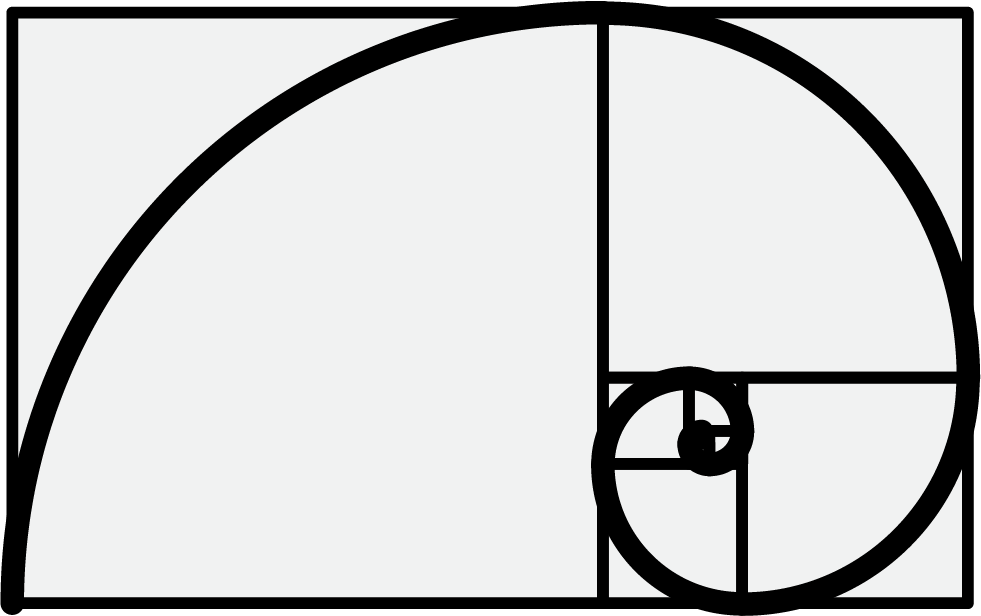
\includegraphics[height=0.75cm]{../../../../AAA_template_latex_settings/pwr-control_logo_doc.png}}
\rfoot{\small Rev.~00}
\geometry{left=2.0cm, right=2.0cm}
\usepackage[european]{circuitikz}
\ctikzset{bipoles/length=1.0cm}

\sisetup{per-mode=symbol}
\setlist{nosep}
\setlength{\parindent}{0pt}
\setlength{\parskip}{3pt}
\allowdisplaybreaks
\renewcommand{\topfraction}{0.9}
\renewcommand{\bottomfraction}{0.9}
\renewcommand{\textfraction}{0.05}
\renewcommand{\floatpagefraction}{0.8}

% --- shorthand ---
\newcommand{\ph}[1]{\underline{#1}}
\newcommand{\Rel}{\mathcal{R}}
\newcommand{\tder}[1]{\frac{\mathrm{d}#1}{\mathrm{d}t}}
\newcommand{\vect}[1]{\boldsymbol{#1}}
\newcommand{\sscname}{\texttt{tri\_monophase\_transformer}}
\newcommand{\one}{\vect{1}}

% =============================================================
%  DOCUMENT DATA (title page: AAA_template_latex_settings/titlepage.tex)
% =============================================================
\newcommand{\DocCategory}{Technical Note}
\newcommand{\DocField}{Power Electronics and Control Systems}
\newcommand{\DocTitle}{%
	{\fontsize{20}{24}\selectfont\bfseries Three-Phase to Single-Phase Transformer} \\[12pt]
	{\fontsize{16}{22}\selectfont\bfseries with two star-connected primaries}
}
\newcommand{\DocSubtitle}{Magnetic model of the three-limb core, steady-state behaviour \\[6pt] and Simscape implementation (\sscname)}
\newcommand{\DocAuthor}{Davide Bagnara}
\newcommand{\DocRevision}{00}
\newcommand{\DocDate}{October 2026}
\newcommand{\DocAbstract}{%
This note derives the model of a transformer with two three-phase star-connected primaries wound on the same three-limb core and one single-phase secondary, the ``tri-monophase'' transformer, and documents the Simscape component \sscname\ of the \texttt{library} repository that implements it. The secondary is described as a series connection of coils on the three limbs with a signed turns distribution $\vect{w}=[w_a,w_b,w_c]$, which covers the line-to-line arrangement ($[1,-1,0]$), the T-type arrangement ($[1,-\tfrac12,-\tfrac12]$) and the single-limb arrangement ($[1,0,0]$). The magnetic circuit of the three-limb core is reduced to a $3\times3$ magnetizing inductance matrix with a positive-sequence and a zero-sequence inductance, the winding equations are written in flux-linkage form with leakage, resistance and a per-limb core-loss branch, and the steady state is worked out: no-load ratio and phase of the output, line currents reflected by the single-phase load, symmetrical components (the negative-sequence current always equals the positive-sequence one), short-circuit impedance ($z_{sc}=z_3+2z_1$ for every distribution without zero sequence), the role of the neutral and of the zero-sequence flux for the single-limb arrangement, the sharing between the two primaries and the circulating current when they are fed by two sources. The per-unit parameterisation, the sign conventions and the limitations of the component are given, and the equations are verified against a numerical re-implementation (Python and MATLAB scripts) in the frequency and in the time domain.
}
\newcommand{\RevisionHistory}{%
	00 & October 2026 & First issue. & \DocAuthor \\
}
\newcommand{\MetaLabelA}{Project Repository}
\newcommand{\MetaValueAUrl}{https://github.com/pwr-control/library.git}
\newcommand{\MetaValueALabel}{library.git}
\newcommand{\MetaLabelB}{Framework}
\newcommand{\MetaValueB}{MATLAB/Simulink/Simscape; Python 3 / NumPy checks}

\begin{document}
% =============================================================
%  pwr-control LaTeX template - FRONTESPIZIO
%
%  Da richiamare come prima istruzione dopo \begin{document}:
%      \input{../../AAA_template_latex_settings/titlepage}
%
%  Il documento deve definire prima di \begin{document}:
%      \DocCategory   categoria del documento
%      \DocField      area tecnica
%      \DocTitle      titolo (una o due righe)
%      \DocSubtitle   sottotitolo
%      \DocAuthor     autore/i, separati da virgola
%      \DocRevision   numero di revisione corrente (es. 00)
%      \DocDate       data della revisione corrente
%      \DocAbstract   abstract
%      \RevisionHistory  righe della tabella di revisione, nel formato
%                        Rev. & Date & Description & Authors \\
%      \MetaLabelA \MetaValueAUrl \MetaValueALabel
%      \MetaLabelB \MetaValueB
% =============================================================

\providecommand{\DocCategory}{Technical Research Report}
\providecommand{\DocField}{Power Electronics and Control Systems}
\providecommand{\DocSubtitle}{}
\providecommand{\DocRevision}{00}
\providecommand{\DocAbstract}{}
\providecommand{\RevisionHistory}{%
	\DocRevision & \DocDate & First issue. & \DocAuthor \\
}

\titlepage

% ---- Intestazione centrata ----
\begin{center}
	{\Large\scshape \DocCategory}\\[8pt]
	{\large\scshape \DocField}
\end{center}

\vspace{30pt plus 4pt minus 14pt}
\noindent\rule{\linewidth}{0.8pt}

% ---- Titolo ----
\begin{center}
	\DocTitle
\end{center}

\vspace{4pt}
\noindent\rule{\linewidth}{2.2pt}

% ---- Sottotitolo ----
\begin{center}
	\begin{onehalfspace}
		{\large\itshape \DocSubtitle}
	\end{onehalfspace}
\end{center}

% ---- Authors / Revision / Date ----
\vspace{30pt plus 4pt minus 14pt}

\noindent
\begin{minipage}[t]{0.46\linewidth}
	\raggedright
	\textbf{Authors:}\\[2pt]
	\DocAuthor
\end{minipage}%
\hfill
\begin{minipage}[t]{0.22\linewidth}
	\centering
	\textbf{Revision:}\\[2pt]
	\DocRevision
\end{minipage}%
\hfill
\begin{minipage}[t]{0.30\linewidth}
	\raggedleft
	\textbf{Date:}\\[2pt]
	\DocDate
\end{minipage}

\vspace{10pt}
\noindent\rule{\linewidth}{0.8pt}

% ---- Abstract ----
\vspace{24pt plus 4pt minus 12pt}

\begin{center}
	\begin{minipage}{0.88\linewidth}
		\footnotesize
		\begin{onehalfspace}
			\textbf{Abstract:} \DocAbstract
		\end{onehalfspace}
	\end{minipage}
\end{center}

\vfill

% ---- Revision history ----
\begin{center}
	\begin{minipage}{0.96\linewidth}
		\centering
		{\footnotesize\scshape Revision history}\\[6pt]
		{\footnotesize
			\begin{tabular}{@{}cl>{\raggedright\arraybackslash}p{0.36\linewidth}>{\raggedright\arraybackslash}p{0.28\linewidth}@{}}
				\toprule
				\textbf{Rev.} & \textbf{Date} & \textbf{Description} & \textbf{Authors} \\
				\midrule
				\RevisionHistory
				\bottomrule
			\end{tabular}}
	\end{minipage}
\end{center}

\vspace{18pt plus 4pt minus 10pt}

% ---- Metadati in fondo ----
\noindent
\begin{tabular}{@{} r @{\quad} l @{}}
	\textsc{\MetaLabelA:} & {\href{\MetaValueAUrl}{\MetaValueALabel}} \\[3pt]
	\textsc{\MetaLabelB:} & {\MetaValueB}       \\[3pt]
\end{tabular}

% =============================================================
%  Fine frontespizio
% =============================================================
\newpage
\pagenumbering{arabic}
\setcounter{page}{1}

\tableofcontents
\newpage
\begin{onehalfspace}

\section*{Nomenclature}
\addcontentsline{toc}{section}{Nomenclature}
Phasors are underlined and refer to rms values; lower-case letters are instantaneous values. Limbs are indexed $k\in\{a,b,c\}$, primaries by $1$ and $2$, the secondary by $3$. Per-unit values are on the single-phase rating $S_r$ and the rated voltages (Section~\ref{sec:pu}).

\begin{onehalfspace}\small
\begin{longtable}{@{}>{$}l<{$} p{11.0cm} l@{}}
\toprule
\text{Symbol} & Description & Unit \\
\midrule
\endfirsthead
\toprule
\text{Symbol} & Description & Unit \\
\midrule
\endhead
N_1,\,N_2 & turns of the primary 1 and primary 2 coil on each limb & -- \\
N_3,\,w_k & reference secondary turns and signed turns distribution: the secondary coil on limb $k$ has $w_k N_3$ turns & -- \\
n_2,\,n_3 & turns ratios $N_2/N_1$ and $N_3/N_1$ & -- \\
g_w & gain of the secondary distribution under balanced flux, $|w_a + a^2 w_b + a\,w_c|$, $a=e^{j120^\circ}$ & -- \\
\kappa_w & reflection factor of the primary impedance, $3\sum_k w_k^2/g_w^2$ & -- \\
\Rel_l,\,\Rel_0 & reluctance of one limb path and of the zero-sequence return path (air, tank, clearances) & \si{\ampere\per\weber} \\
\Phi_k,\,\psi_k & flux of limb $k$ and flux linkage of the primary-1 coil on limb $k$, $\psi_k=N_1\Phi_k$ & \si{\weber}, \si{\volt\second} \\
i_{1k},\,i_{2k},\,i_3 & currents of the primary coils (into the line terminal) and of the secondary (out of $s_1$) & \si{\ampere} \\
i_{m,k},\,i_{fe,k} & magnetizing and core-loss current of limb $k$, referred to primary 1 & \si{\ampere} \\
L_m,\,L_{m0} & positive-sequence and zero-sequence magnetizing inductance, referred to primary 1 & \si{\henry} \\
R_1,L_1;\,R_2,L_2;\,R_3,L_3 & resistance and leakage inductance of one primary-1 coil, one primary-2 coil, the whole secondary & \si{\ohm}, \si{\henry} \\
R_{fe} & core-loss resistance per limb, referred to primary 1 & \si{\ohm} \\
S_r,\,V_1,\,V_2,\,V_3,\,f_r & rated apparent power (single-phase output), rated line-to-line voltages of the primaries, rated secondary voltage, rated frequency & \si{\volt\ampere}, \si{\volt}, \si{\hertz} \\
Z_{b1},\,Z_{b2},\,Z_{b3} & base impedances $V_1^2/S_r$, $V_2^2/S_r$, $V_3^2/S_r$ & \si{\ohm} \\
z_1,\,z_2,\,z_3 & per-unit coil impedances $r+jl$ & \si{\pu} \\
\ph{I}_0,\,\ph{I}_+,\,\ph{I}_- & zero, positive and negative sequence components of the line currents & \si{\ampere} \\
\bottomrule
\end{longtable}
\end{onehalfspace}

\section{Introduction}

The transformer considered here has \emph{two} three-phase primaries, both star-connected, and \emph{one} single-phase secondary. Such a unit is met when two three-phase sources, for instance two converters or two generators, have to feed one single-phase load through a common magnetic circuit, with galvanic separation between the sources and between the sources and the load; the two primaries can also be put in series or in parallel to obtain a dual-voltage input. The device is simple to use but not obvious to understand: the single-phase load is intrinsically unbalanced for the three-phase sources, the way the load current distributes among the three lines depends on how the secondary coils sit on the limbs of the core, and the star connection without neutral forbids some arrangements altogether. The purpose of this note is to settle these points with a model that can be simulated, the Simscape component \sscname\ added to the \texttt{library} repository.

The model rests on four assumptions, stated here because they fix the topology; the open points that should be confirmed on the real unit are listed in Section~\ref{sec:conclusions}.
\begin{enumerate}
\item \textbf{One three-limb core.} Both primaries and the secondary are wound on the same three-limb core, one limb per phase. A bank of three single-phase units and a five-limb core are recovered by a parameter (the zero-sequence magnetizing inductance equal to the positive-sequence one).
\item \textbf{Both primaries in star, no displacement.} The two primaries are star-connected with the same winding sense on each limb, so their phase voltages are in phase (vector group Yy0). Both neutrals are brought out as ports and can be left floating, grounded or tied together.
\item \textbf{Secondary as a series of limb coils.} The single-phase secondary is the series connection of coils wound on the limbs, with $w_k N_3$ turns on limb $k$; the sign of $w_k$ is the winding sense. The three practical arrangements are the line-to-line one, $\vect{w}=[1,-1,0]$, the T-type one, $\vect{w}=[1,-\tfrac12,-\tfrac12]$, and the single-limb one, $\vect{w}=[1,0,0]$.
\item \textbf{Linear magnetics.} No saturation, no hysteresis; the core loss is a linear resistance per limb.
\end{enumerate}

\section{Winding arrangement and magnetic circuit}

\subsection{Arrangement}

Figure~\ref{fig:arr} shows the arrangement. Each limb $k$ carries three coils: the primary-1 coil with $N_1$ turns, the primary-2 coil with $N_2$ turns and the secondary coil with $w_k N_3$ turns. The primary-1 coils are joined at the neutral $N_1$ and their line terminals are $A_1$, $B_1$, $C_1$; likewise for primary 2. The secondary coils are connected in series between $s_1$ and $s_2$; a coil with $w_k<0$ is connected with its winding sense reversed, a coil with $w_k=0$ is absent.

\begin{figure}[htbp]
\centering
\resizebox{\linewidth}{!}{%
\begin{tikzpicture}[scale=0.9, every node/.style={font=\small}]
% core
\draw[line width=3pt, gray!60] (0,0) rectangle (8,5.2);
\draw[line width=3pt, gray!60] (4,0) -- (4,5.2);
\foreach \x/\lab in {0/a, 4/b, 8/c} {
  \node[gray!80!black] at (\x,5.55) {limb $\lab$};
  % primary 1 coil
  \draw[thick, blue!70!black] (\x-0.35,4.5) rectangle (\x+0.35,3.6);
  \node[blue!70!black, anchor=west] at (\x+0.45,4.05) {$N_1$};
  % primary 2 coil
  \draw[thick, red!70!black] (\x-0.35,3.1) rectangle (\x+0.35,2.2);
  \node[red!70!black, anchor=west] at (\x+0.45,2.65) {$N_2$};
  % secondary coil
  \draw[thick, green!50!black] (\x-0.35,1.7) rectangle (\x+0.35,0.8);
}
\node[green!50!black, anchor=west] at (0.45,1.25) {$w_a N_3$};
\node[green!50!black, anchor=west] at (4.45,1.25) {$w_b N_3$};
\node[green!50!black, anchor=west] at (8.45,1.25) {$w_c N_3$};
\node[anchor=south] at (4,-0.9) {\footnotesize three-limb core: fluxes $\Phi_a$, $\Phi_b$, $\Phi_c$ in the limbs, $\Phi_a+\Phi_b+\Phi_c$ returns outside the core};
% electrical connection sketch on the right
\begin{scope}[xshift=11.2cm, yshift=0.0cm]
\node[anchor=south] at (1.6,5.4) {\footnotesize primary 1 (star)};
\draw[blue!70!black] (1.6,4.3) -- (1.6,5.1) node[above]{$A_1$};
\draw[blue!70!black] (1.6,4.3) -- (0.5,3.6) -- (0.2,3.4) node[left]{$B_1$};
\draw[blue!70!black] (1.6,4.3) -- (2.7,3.6) -- (3.0,3.4) node[right]{$C_1$};
\fill[blue!70!black] (1.6,4.3) circle (1.3pt);
\node[blue!70!black, anchor=north] at (1.6,4.2) {$N_1$};
\node[anchor=south] at (1.6,2.55) {\footnotesize primary 2 (star)};
\draw[red!70!black] (1.6,1.45) -- (1.6,2.25) node[above]{$A_2$};
\draw[red!70!black] (1.6,1.45) -- (0.5,0.75) -- (0.2,0.55) node[left]{$B_2$};
\draw[red!70!black] (1.6,1.45) -- (2.7,0.75) -- (3.0,0.55) node[right]{$C_2$};
\fill[red!70!black] (1.6,1.45) circle (1.3pt);
\node[red!70!black, anchor=north] at (1.6,1.35) {$N_2$};
\end{scope}
\begin{scope}[xshift=11.2cm, yshift=-1.9cm]
\node[anchor=south] at (1.6,0.75) {\footnotesize secondary (series)};
\draw[green!50!black] (-0.3,0.3) node[left]{$s_1$} -- (0.2,0.3)
  to[L, l_=$w_a N_3$] (1.2,0.3) to[L, l_=$w_b N_3$] (2.2,0.3) to[L, l_=$w_c N_3$] (3.2,0.3) -- (3.6,0.3) node[right]{$s_2$};
\end{scope}
\end{tikzpicture}}
\caption{Coils on the three limbs (left) and electrical connections (right). The two primaries are stars with the neutrals $N_1$, $N_2$ brought out; the secondary is the series connection of the limb coils with the signed turns distribution $\vect{w}=[w_a,w_b,w_c]$.}
\label{fig:arr}
\end{figure}

\subsection{Magnetic circuit of the three-limb core}

Let $\Phi_k$ be the flux of limb $k$, counted from the bottom to the top yoke, and let the limb path (limb plus its share of the yokes) have reluctance $\Rel_l$. The three limbs are in parallel between the two yokes, so the magnetic potential difference $u$ between the yokes is the same for the three of them:
\begin{equation}
\mathcal{F}_k - \Rel_l\,\Phi_k = u , \qquad k = a,b,c ,
\label{eq:limb}
\end{equation}
where $\mathcal{F}_k$ is the total magneto-motive force on limb $k$. The sum of the three limb fluxes cannot close inside the core: it returns from the top to the bottom yoke through the air, the tank and the clearances, a path of reluctance $\Rel_0$,
\begin{equation}
u = \Rel_0\,(\Phi_a + \Phi_b + \Phi_c) .
\label{eq:zero}
\end{equation}
Eliminating $u$ and writing $\vect{\Phi}=[\Phi_a,\Phi_b,\Phi_c]^T$,
\begin{equation}
\vect{\mathcal{F}} = \left(\Rel_l\,\mathbf{I} + \Rel_0\,\one\one^T\right)\vect{\Phi}
\quad\Longrightarrow\quad
\vect{\Phi} = \frac{1}{\Rel_l}\left(\mathbf{I} - \frac{\Rel_0}{\Rel_l + 3\Rel_0}\,\one\one^T\right)\vect{\mathcal{F}} ,
\label{eq:magcirc}
\end{equation}
with $\one=[1,1,1]^T$ (Sherman--Morrison). The mutual term is negative: the flux produced on one limb returns in part through the other two. With the magneto-motive forces referred to primary 1, $\mathcal{F}_k = N_1 i_{m,k}$, and the flux linkages of the primary-1 coils, $\psi_k = N_1\Phi_k$,
\begin{equation}
\boxed{\;\vect{\psi} = \mathbf{L}_\mu\,\vect{i}_m , \qquad
\mathbf{L}_\mu = L_m\,\mathbf{I} - \frac{L_m - L_{m0}}{3}\,\one\one^T , \qquad
L_m = \frac{N_1^2}{\Rel_l}, \quad L_{m0} = \frac{N_1^2}{\Rel_l + 3\Rel_0} .\;}
\label{eq:Lmu}
\end{equation}
The eigenvectors of $\mathbf{L}_\mu$ are the symmetrical components: the positive and the negative sequence see $L_m$, the zero sequence sees $L_{m0}$. Two limiting cases fix the meaning of $L_{m0}$. For a bank of three single-phase units, or a five-limb core, the zero-sequence flux has an iron return path, $\Rel_0\to0$ and $L_{m0}=L_m$: the three limbs are decoupled. For a three-limb core $\Rel_0\gg\Rel_l$ and $L_{m0}\ll L_m$, typically a fraction of a per unit against the tens or hundreds of per unit of $L_m$; it is measured with the zero-sequence open-circuit test, the three primary coils in parallel fed by a single-phase source against the neutral.

\section{Electrical equations}

\subsection{Winding equations}

Each coil is described by its resistance, its leakage inductance, lumped in series and not coupled to the other coils, and the voltage induced by the limb flux. Taking the current of the primary coils as entering at the line terminal and leaving at the neutral, and the secondary current as leaving $s_1$ (generator convention):
\begin{align}
v_{A1} - v_{N1} &= R_1\, i_{1a} + L_1\,\tder{i_{1a}} + \tder{\psi_a}, &
v_{A2} - v_{N2} &= R_2\, i_{2a} + L_2\,\tder{i_{2a}} + n_2\,\tder{\psi_a}, \notag\\
v_{B1} - v_{N1} &= R_1\, i_{1b} + L_1\,\tder{i_{1b}} + \tder{\psi_b}, &
v_{B2} - v_{N2} &= R_2\, i_{2b} + L_2\,\tder{i_{2b}} + n_2\,\tder{\psi_b}, \label{eq:prim}\\
v_{C1} - v_{N1} &= R_1\, i_{1c} + L_1\,\tder{i_{1c}} + \tder{\psi_c}, &
v_{C2} - v_{N2} &= R_2\, i_{2c} + L_2\,\tder{i_{2c}} + n_2\,\tder{\psi_c}, \notag
\end{align}
\begin{equation}
v_{s1} - v_{s2} = e_3 - R_3\, i_3 - L_3\,\tder{i_3}, \qquad
e_3 = n_3\left(w_a\,\tder{\psi_a} + w_b\,\tder{\psi_b} + w_c\,\tder{\psi_c}\right),
\label{eq:sec}
\end{equation}
with $n_2 = N_2/N_1$ and $n_3 = N_3/N_1$. The secondary induced voltage $e_3$ is the sum of the limb voltages weighted by the distribution.

\subsection{Magneto-motive force balance and core loss}

The net magneto-motive force of limb $k$ is the sum of the ampere-turns of the three coils on it. The core loss is represented by a resistance $R_{fe}$ per limb across the limb voltage $\mathrm{d}\psi_k/\mathrm{d}t$, and its current is taken out of the magnetizing ampere-turns, as in the usual T equivalent:
\begin{equation}
i_{m,k} = i_{1k} + n_2\, i_{2k} - n_3\, w_k\, i_3 - \frac{1}{R_{fe}}\tder{\psi_k}, \qquad k=a,b,c .
\label{eq:mmf}
\end{equation}
The minus sign on $i_3$ follows from the generator convention of the secondary. Equations \eqref{eq:Lmu}, \eqref{eq:prim}, \eqref{eq:sec} and \eqref{eq:mmf} are the complete model: ten differential variables (the seven coil currents and the three flux linkages, of which the seven coil currents are states through the leakage inductances and the three flux linkages through $\mathbf{L}_\mu$) and three algebraic magnetizing currents. Kirchhoff's current law at the neutrals is not part of the model: it is imposed by whatever is connected to $N_1$ and $N_2$, so an isolated star ($\sum_k i_{1k}=0$) and a grounded one are both covered.

\subsection{Matrix form}

With $\vect{i}_1$, $\vect{i}_2$ the primary coil-current vectors, $\vect{v}_1 = [v_{A1},v_{B1},v_{C1}]^T - v_{N1}\one$ and $\vect{v}_2$ likewise, the model reads
\begin{equation}
\begin{aligned}
\vect{v}_1 &= R_1\,\vect{i}_1 + L_1\,\tder{\vect{i}_1} + \tder{\vect{\psi}}, &
\vect{v}_2 &= R_2\,\vect{i}_2 + L_2\,\tder{\vect{i}_2} + n_2\tder{\vect{\psi}}, &
v_3 &= n_3\,\vect{w}^T\tder{\vect{\psi}} - R_3\,i_3 - L_3\,\tder{i_3},\\
\vect{\psi} &= \mathbf{L}_\mu\left(\vect{i}_1 + n_2\,\vect{i}_2 - n_3\,\vect{w}\,i_3 - \frac{1}{R_{fe}}\tder{\vect{\psi}}\right),
\end{aligned}
\label{eq:matrix}
\end{equation}
which is the flux-linkage form of a seven-winding transformer whose $7\times7$ inductance matrix has the magnetizing part $\mathbf{T}\,\mathbf{L}_\mu\,\mathbf{T}^T$ with $\mathbf{T}=[\mathbf{I};\, n_2\mathbf{I};\, -n_3\vect{w}^T]$ and the leakage part $\mathrm{diag}(L_1\one, L_2\one, L_3)$. The magnetizing part has rank three, one magnetizing degree of freedom per limb, which is what distinguishes this unit from a bank of seven independent coils.

\section{Steady-state behaviour}

\subsection{No load: output voltage and phase}

Let primary 1 be supplied by a balanced positive-sequence set of phase voltages $\ph{V}_A = V_1/\sqrt3\angle0^\circ$, $\ph{V}_B = \ph{V}_A a^2$, $\ph{V}_C = \ph{V}_A a$, with $a = e^{j120^\circ}$. Neglecting the drop on $R_1$, $L_1$, the limb flux linkages are $\ph{\Psi}_k = \ph{V}_k/(j\omega)$: a balanced positive-sequence set, which drives no zero-sequence flux whatever $L_{m0}$. The secondary induced voltage is then
\begin{equation}
\ph{E}_3 = n_3\left(w_a + a^2 w_b + a\,w_c\right)\ph{V}_A = n_3\,\ph{W}\,\ph{V}_A ,
\qquad g_w = |\ph{W}| = \sqrt{\left(w_a - \tfrac{w_b+w_c}{2}\right)^2 + \tfrac34\left(w_c - w_b\right)^2} .
\label{eq:E3}
\end{equation}
The no-load secondary voltage is $V_3 = n_3\,g_w\,V_1/\sqrt3$, and $\arg\ph{W}$ is its phase with respect to $\ph{V}_A$. Table~\ref{tab:distr} gives the three practical distributions. The gain obeys the identity
\begin{equation}
g_w^2 = \tfrac32\sum_k w_k^2 - \tfrac12\Big(\sum_k w_k\Big)^2 ,
\label{eq:gw}
\end{equation}
so for a distribution without zero sequence ($\sum_k w_k=0$) $g_w^2 = \tfrac32\sum_k w_k^2$. The turns ratio that gives the rated secondary voltage is therefore
\begin{equation}
\boxed{\;n_3 = \frac{N_3}{N_1} = \frac{\sqrt3\,V_3}{g_w\,V_1}\;}
\label{eq:n3}
\end{equation}
and this is how the component derives it from the nameplate voltages.

\begin{table}[htbp]
\centering
\caption{The three practical secondary distributions under a balanced positive-sequence supply (ideal transformer). $\ph{I}_A$, $\ph{I}_B$, $\ph{I}_C$ are the primary-1 line currents reflected by the secondary current $\ph{I}_3$.}
\label{tab:distr}
\footnotesize
\begin{tabular}{l p{4.6cm} c c p{5.6cm}}
\toprule
$\vect{w}$ & arrangement & $g_w$ & $\arg\ph{W}$ (ref. $\ph{V}_A$) & reflected line currents \\
\midrule
$[1,-1,0]$ & coils on $a$ and $b$ in opposition, output $\propto \ph{V}_{AB}$ & $\sqrt3$ & $+30^\circ$ & $\ph{I}_A = -\ph{I}_B = n_3\ph{I}_3$, $\ph{I}_C = 0$ \\
$[1,-\tfrac12,-\tfrac12]$ & T type, output $\propto \ph{V}_A$ & $\tfrac32$ & $0^\circ$ & $\ph{I}_A = n_3\ph{I}_3$, $\ph{I}_B = \ph{I}_C = -\tfrac12 n_3\ph{I}_3$ \\
$[1,0,0]$ & coil on limb $a$ only, output $\propto \ph{V}_A$ & $1$ & $0^\circ$ & $\ph{I}_A = n_3\ph{I}_3$, $\ph{I}_B = \ph{I}_C = 0$, neutral current $n_3\ph{I}_3$ \\
\bottomrule
\end{tabular}
\end{table}

\begin{figure}[htbp]
\centering
\begin{tikzpicture}[scale=1.6,>=stealth]
\draw[->,gray]  (0,0) -- (0:1)      node[right]{$\ph{V}_{A}$};
\draw[->,gray]  (0,0) -- (-120:1)   node[below]{$\ph{V}_{B}$};
\draw[->,gray]  (0,0) -- (120:1)    node[left]{$\ph{V}_{C}$};
\draw[->,thick,blue!70!black] (0,0) -- (30:1.732) node[right]{$\ph{E}_3/n_3$, $\vect{w}=[1,-1,0]$ ($=\ph{V}_{AB}$)};
\draw[->,thick,green!50!black] (0,0) -- (0:1.5) node[below right]{$\ph{E}_3/n_3$, $\vect{w}=[1,-\tfrac12,-\tfrac12]$};
\draw (0:0.5) arc (0:30:0.5);
\node at (15:0.68) {\footnotesize $30^\circ$};
\end{tikzpicture}
\caption{No-load phasors: the line-to-line distribution gives an output in phase with $\ph{V}_{AB}$ and $\sqrt3$ times the phase voltage per unit turns ratio; the T-type distribution gives an output in phase with $\ph{V}_A$ and $3/2$ times the phase voltage.}
\label{fig:phasor}
\end{figure}

\subsection{Load: reflected line currents and the role of the neutral}

With the magnetizing current neglected, \eqref{eq:mmf} gives for primary 1 alone
\begin{equation}
i_{1k} = n_3\,w_k\,i_3 + i_{0}, \qquad k=a,b,c ,
\label{eq:refl}
\end{equation}
where $i_0$ is a common term allowed by the magnetic circuit only if it can flow: it is the zero-sequence current. For an isolated star $\sum_k i_{1k}=0$, hence $3i_0 = -n_3 i_3\sum_k w_k$. If the distribution has no zero sequence, $i_0=0$ and the line currents are exactly $n_3 w_k i_3$: the single-phase load current is mapped onto the lines with the same pattern as the secondary turns (Table~\ref{tab:distr}, Figure~\ref{fig:lines}). If the distribution has a zero sequence, as the single-limb one, the ampere-turns $n_3 i_3 \sum_k w_k/3$ on each limb remain uncompensated and must be balanced by zero-sequence magnetizing current, which the floating star cannot supply through the lines: the ampere-turns are then balanced by the zero-sequence flux, $\psi_0 = L_{m0}\,i_{m,0}$ with $i_{m,0} = -n_3 i_3\sum_k w_k/3$. This flux adds to all three limbs, the loaded limb is partly demagnetised and the other two over-fluxed, and the output voltage becomes soft: with the default parameters of Section~\ref{sec:pu} ($l_{m0}=\SI{0.5}{\pu}$) the rated resistive load on $\vect{w}=[1,0,0]$ with floating neutral brings the output to \SI{196}{V} instead of \SI{224}{V} and the flux of limb $b$ to \SI{1.40}{\pu} (Section~\ref{sec:verif}). In a real core the over-fluxed limbs saturate, the zero-sequence inductance collapses and the output collapses with it; the arrangement is usable only with the neutral connected, in which case $i_0 = n_3 i_3\sum_k w_k/3$ flows in the neutral and the three lines carry $n_3 w_k i_3$.

\subsection{Symmetrical components}

For a distribution without zero sequence, \eqref{eq:refl} gives
\begin{equation}
\ph{I}_+ = \tfrac13\left(\ph{I}_A + a\ph{I}_B + a^2\ph{I}_C\right) = \tfrac13\,n_3\,\ph{I}_3\,\ph{W}^{*}, \qquad
\ph{I}_- = \tfrac13\,n_3\,\ph{I}_3\,\ph{W}, \qquad \ph{I}_0 = 0 ,
\label{eq:seq}
\end{equation}
so $|\ph{I}_-| = |\ph{I}_+| = n_3 g_w I_3/3$ whatever the distribution. This is not a defect of a particular connection but the signature of the single-phase load: its instantaneous power pulsates at twice the line frequency, and a three-phase source can deliver a pulsating power only through a negative-sequence current of the same magnitude as the positive-sequence one. No passive transformer connection can balance a single-phase load on a three-phase system; the distribution only decides \emph{which} lines carry the current. At rated load $|\ph{I}_+| = S_r/(\sqrt3 V_1)$, the three-phase base current.

\subsection{Short-circuit impedance and copper loss}

With the secondary shorted and primary 1 supplied, the limb voltages are $\ph{E}_k = \ph{V}_k - \ph{V}_{N1} - Z_1\ph{I}_{1k}$ with $Z_1 = R_1 + j\omega L_1$, and $\ph{E}_3 = n_3\sum_k w_k\ph{E}_k$. For a distribution without zero sequence the neutral potential drops out and, with \eqref{eq:refl},
\begin{equation}
\ph{E}_3 = n_3\,\ph{V}_w - n_3^2 Z_1 \Big(\sum_k w_k^2\Big)\ph{I}_3 , \qquad \ph{V}_w = \sum_k w_k \ph{V}_k ,
\end{equation}
i.e. the secondary sees the Th\'evenin voltage $n_3\ph{V}_w$ (the rated voltage at rated supply) behind the impedance
\begin{equation}
Z_{sc} = Z_3 + n_3^2\Big(\sum_k w_k^2\Big) Z_1
\qquad\Longrightarrow\qquad
z_{sc} = z_3 + \kappa_w\, z_1 , \quad \kappa_w = \frac{3\sum_k w_k^2}{g_w^2} ,
\label{eq:zsc}
\end{equation}
in per unit on the bases of Section~\ref{sec:pu}. By \eqref{eq:gw}, $\kappa_w = 2$ for \emph{every} distribution without zero sequence: the reflected primary impedance, hence the short-circuit impedance, the voltage regulation and the primary copper loss at a given load, do not depend on whether the coils sit on two limbs or on three. The copper loss of primary 1 at rated load is $\kappa_w r_1 = 2r_1$ per unit in both cases: the T-type arrangement loads line $A$ with the full reflected current and lines $B$, $C$ with one half, but with a turns ratio $2/\sqrt3$ higher, and $I_A^2 + 2(I_A/2)^2$ equals $2I^2$ of the line-to-line arrangement. With the neutral connected the same expression holds for a distribution with zero sequence, with $\kappa_w$ from \eqref{eq:gw}: $\kappa_w = 3$ for $\vect{w}=[1,0,0]$, since the whole load current flows through one coil at the phase voltage. When primary 2 is in parallel with primary 1 on the same source, $z_1$ is replaced by the parallel $z_1 z_2/(z_1+z_2)$ (for $V_2 = V_1$).

The practical consequence for the parameterisation is that a nameplate short-circuit voltage $u_{cc}$ measured from the secondary with one primary supplied corresponds to $|z_3 + 2z_1| = u_{cc}$; splitting it evenly, $l_1 = l_3 = u_x/3$ and $r_1 = r_3 = u_r/3$, is a reasonable default when the individual coil values are unknown.

\subsection{Two primaries}

\textbf{In parallel on the same source.} Each primary carries the fraction of the reflected current given by the admittance divider $z_2/(z_1+z_2)$, one half for identical windings, and the short-circuit impedance drops to $z_3 + 2 z_1 z_2/(z_1+z_2)$.

\textbf{Fed by two sources.} If the two primaries are fed by two sources of the same amplitude displaced by an angle $\delta$, with the secondary open, a circulating current flows through the two leakage impedances in series: per phase
\begin{equation}
\ph{I}_{circ} = \frac{\ph{V}_1 - \ph{V}_2}{Z_1 + Z_2} , \qquad
\frac{I_{circ}}{I_{b1}} = \frac{2\sin(\delta/2)}{|z_1+z_2|} .
\label{eq:circ}
\end{equation}
It is balanced, so it does not involve the neutrals or the zero-sequence inductance, and it is large: with $z_1 + z_2 = 0.01 + j0.06$ per unit, a displacement of $2^\circ$ gives \SI{0.57}{\pu} and $5^\circ$ gives \SI{1.43}{\pu}. Two converters feeding the two primaries must therefore be synchronised tightly or share the current through their control; the transformer provides galvanic separation between them, not decoupling.

\section{Simscape component}
\label{sec:ssc}

The component \sscname\ (package \path{+tri_monophase_transformer} in the folder \path{library/foundation/electrical_machines}) implements \eqref{eq:Lmu}, \eqref{eq:prim}, \eqref{eq:sec} and \eqref{eq:mmf} without reformulation. Its ports are the eight primary nodes \texttt{A1}, \texttt{B1}, \texttt{C1}, \texttt{N1}, \texttt{A2}, \texttt{B2}, \texttt{C2}, \texttt{N2} on the left, the two secondary nodes \texttt{s1}, \texttt{s2} on the right, and three physical-signal outputs \texttt{psi\_a}, \texttt{psi\_b}, \texttt{psi\_c}, the flux linkages of the primary-1 coils, which show directly which limbs are loaded and whether a zero-sequence flux is present. A neutral left unconnected is an isolated star; connecting \texttt{N1} to \texttt{N2} or to the source neutral is done outside the block.

\subsection{Parameters and per-unit bases}
\label{sec:pu}

The parameters are listed in Table~\ref{tab:par}. The impedances are entered in per unit on the single-phase rating $S_r$ and on the rated voltages:
\begin{equation}
Z_{b1} = \frac{V_1^2}{S_r}, \qquad Z_{b2} = \frac{V_2^2}{S_r}, \qquad Z_{b3} = \frac{V_3^2}{S_r}, \qquad \omega_r = 2\pi f_r ,
\end{equation}
so that $R_1 = r_1 Z_{b1}$, $L_1 = l_1 Z_{b1}/\omega_r$ refer to one coil of the primary-1 star on the usual three-phase base of a transformer of rating $S_r$ and line-to-line voltage $V_1$; likewise for primary 2 and for the secondary, whose $R_3$, $L_3$ are those of the whole winding. The magnetizing inductances and the core-loss resistance are referred to primary 1: $L_m = l_m Z_{b1}/\omega_r$, $L_{m0} = l_{m0} Z_{b1}/\omega_r$, $R_{fe} = r_{fe} Z_{b1}$. With $l_m = 100$ the no-load current is $1/100$ of the three-phase base current $S_r/(\sqrt3 V_1)$. The turns ratios are not entered: $n_2 = V_2/V_1$, and $n_3$ from \eqref{eq:n3}, with $g_w$ computed from $\vect{w}$ by \eqref{eq:E3}; the component asserts $g_w>0$, since a distribution such as $[1,1,1]$ would give no fundamental output at all.

\begin{table}[htbp]
\centering
\caption{Parameters of the \sscname\ component.}
\label{tab:par}
\small
\begin{tabular}{llll}
\toprule
Name & Description & Unit & Default \\
\midrule
\texttt{Sr}  & rated apparent power (single-phase output) & \si{\volt\ampere} & \num{100e3} \\
\texttt{V1}  & primary 1 rated line-to-line voltage, rms & \si{\volt} & 400 \\
\texttt{V2}  & primary 2 rated line-to-line voltage, rms & \si{\volt} & 400 \\
\texttt{V3}  & secondary rated voltage, rms & \si{\volt} & 230 \\
\texttt{fr}  & rated frequency & \si{\hertz} & 50 \\
\texttt{ws}  & secondary turns distribution on limbs $a$, $b$, $c$, $[w_a\;w_b\;w_c]$ & -- & \texttt{[1 -1 0]} \\
\texttt{r1}, \texttt{l1} & resistance and leakage inductance of one primary-1 coil & pu & 0.005, 0.030 \\
\texttt{r2}, \texttt{l2} & resistance and leakage inductance of one primary-2 coil & pu & 0.005, 0.030 \\
\texttt{r3}, \texttt{l3} & resistance and leakage inductance of the secondary & pu & 0.005, 0.030 \\
\texttt{lm}  & positive-sequence magnetizing inductance & pu & 100 \\
\texttt{lm0} & zero-sequence magnetizing inductance & pu & 0.5 \\
\texttt{rfe} & core-loss resistance per limb & pu & 500 \\
\bottomrule
\end{tabular}
\end{table}

The default $l_{m0} = 0.5$ is a placeholder for a three-limb core, to be replaced by the measured value; set $l_{m0} = l_m$ for a bank of single-phase units or a five-limb core. It plays no role as long as the secondary distribution has no zero sequence and the neutrals carry no current, which is the default situation.

\subsection{Implemented equations and sign conventions}

With the variables of the component, \texttt{i1a}$\ldots$\texttt{i2c} the coil currents from the line terminals to the neutrals, \texttt{i3} the secondary current out of \texttt{s1}, \texttt{psia}, \texttt{psib}, \texttt{psic} the flux linkages and \texttt{ima}, \texttt{imb}, \texttt{imc} the magnetizing currents, the equations block reads
\begin{align*}
&\texttt{A1.v - N1.v == R1*i1a + L1*der(i1a) + der(psia);} \quad\text{(and } B1, C1\text{)}\\
&\texttt{A2.v - N2.v == R2*i2a + L2*der(i2a) + n2*der(psia);} \quad\text{(and } B2, C2\text{)}\\
&\texttt{s1.v - s2.v == n3*(ws(1)*der(psia) + ws(2)*der(psib) + ws(3)*der(psic))}\\
&\qquad\qquad\qquad\texttt{- R3*i3 - L3*der(i3);}\\
&\texttt{ima == i1a + n2*i2a - n3*ws(1)*i3 - der(psia)/Rfe;} \quad\text{(and } b, c\text{)}\\
&\texttt{psia == Lm*ima - Lc*(ima + imb + imc);} \quad\text{(and } b, c\text{)}, \qquad \texttt{Lc = (Lm - Lm0)/3}.
\end{align*}
The branches are \texttt{A1.i -> N1.i} and so on for the six primary coils, and \texttt{s2.i -> s1.i} for the secondary. Positive current therefore enters the block at the primary line terminals and leaves it at \texttt{s1}; with a positive-sequence $A$--$B$--$C$ supply and the default distribution, \texttt{s1.v - s2.v} is in phase with $v_{A1}-v_{B1}$. Reversing the sign of all the entries of \texttt{ws} reverses the secondary polarity, which is the simplest polarity check.

\subsection{Limitations}

The magnetic model is linear: saturation, hysteresis, inrush and the frequency dependence of the core loss are not represented, the leakage inductances are not mutually coupled and there is no thermal port. The zero-sequence inductance is a constant, whereas in a three-limb core it depends on the tank and on the flux level; it should be measured for the actual unit if the zero-sequence behaviour matters. The component is not a replacement for a detailed design model of the core: it answers the questions of this note, namely ratio, phase, line currents, regulation and the interaction between the two primaries.

\subsection{Building the library block}

The block library \texttt{tri\_monophase\_transformer\_lib.slx} is built, as for every component of the repository, from the folder that contains the package:
\begin{verbatim}
cd library/foundation/electrical_machines
ssc_build tri_monophase_transformer
\end{verbatim}

\section{Verification}
\label{sec:verif}

The equations of the component were re-implemented as a linear descriptor system $\mathbf{E}\dot{\vect{x}} = \mathbf{A}\vect{x} + \mathbf{B}\vect{u}$ in the twelve unknowns (seven coil currents, three flux linkages, two neutral potentials) with the primary-1 terminals fed by an ideal balanced source and the secondary open, shorted or loaded by the rated resistance $V_3^2/S_r$. The system is solved in the frequency domain, $(j\omega\mathbf{E}-\mathbf{A})\ph{\vect{X}} = \mathbf{B}\ph{\vect{U}}$, by the companion script \texttt{tri\_monophase\_transformer\_check.py} and by \texttt{test\_tri\_monophase\_transformer.m} shipped with the component; the Python script also integrates it in the time domain with the trapezoidal rule and draws the figures. The results for the default parameters are in Table~\ref{tab:verif}; the expected values are the closed forms of Section~4.

\begin{table}[htbp]
\centering
\caption{Steady-state checks with the default parameters of Table~\ref{tab:par} ($I_{3n} = S_r/V_3 = \SI{434.8}{A}$, $I_{b1} = S_r/(\sqrt3 V_1) = \SI{144.3}{A}$). The power balance $P_{in} = P_{out} + P_{cu} + P_{fe}$ closes to numerical precision in every case.}
\label{tab:verif}
\small
\begin{tabular}{p{5.3cm}p{5.1cm}p{5.1cm}}
\toprule
Test & Model & Expected \\
\midrule
1. No load, $V_1$ on primary 1 & $V_3 = \SI{229.93}{V}$ in phase with $\ph{V}_{AB}$, $I_1 = \SI{1.472}{A}$, open-circuit $V_2 = \SI{399.9}{V}$ & $V_3 = \SI{230}{V}$, $I_1 = \sqrt{(I_{b1}/l_m)^2 + (V_1/\sqrt3/(r_{fe}Z_{b1}))^2} = \SI{1.472}{A}$ \\
2. Rated resistive load & $V_3 = \SI{225.65}{V}$, $I_3 = \SI{426.6}{A}$, $I_A = \SI{244.8}{A}$, $I_B = \SI{246.3}{A}$, $I_C = \SI{1.5}{A}$, $|\ph{I}_+| = \SI{142.0}{A}$, $|\ph{I}_-| = \SI{141.6}{A}$ & $V_3 = V_{3n}/|1 + z_3 + 2z_1| = \SI{225.7}{V}$, $I_A = I_B = n_3 I_3 = \SI{245.3}{A}$, $I_C$ magnetizing only, $|\ph{I}_-| = |\ph{I}_+|$ \\
3. Secondary short circuit & $z_{sc} = I_{3n}/I_3 = \SI{0.0913}{\pu}$ & $|z_3 + 2z_1| = \SI{0.0912}{\pu}$ \\
4. Primaries in parallel, short circuit & $z_{sc} = \SI{0.0608}{\pu}$; at rated load each primary carries \SI{123.3}{A} on $A$ & $|z_3 + 2 z_1 z_2/(z_1+z_2)| = \SI{0.0608}{\pu}$; equal sharing \\
5. Second source displaced by $2^\circ$ / $5^\circ$, no load & $I_{circ}/I_{b1} = 0.574$ / $1.434$ & $2\sin(\delta/2)/|z_1+z_2| = 0.574$ / $1.434$ \\
6. $\vect{w} = [1,-\tfrac12,-\tfrac12]$, rated load & $V_3 = \SI{225.65}{V}$ at $-35.1^\circ$ from $\ph{V}_{AB}$, $I_A = \SI{283.5}{A}$, $I_B = \SI{143.0}{A}$, $I_C = \SI{140.6}{A}$, $z_{sc} = \SI{0.0913}{\pu}$ & same $V_3$ and $z_{sc}$ as test 2, phase $-30^\circ$ minus the load angle, $I_A = 2I_B = 2I_C$ \\
7. $\vect{w} = [1,0,0]$, rated load, $N_1$ floating & $V_3 = \SI{195.8}{V}$; limb flux linkages $0.86$, $1.40$, $0.87$ pu & output soft and limb $b$ over-fluxed by the zero-sequence flux $l_{m0}\,i_{m,0}$ \\
\phantom{7.} same, $N_1$ grounded & $V_3 = \SI{224.0}{V}$, $I_A = \SI{414.2}{A}$, $I_B$, $I_C < \SI{10}{A}$, $|\ph{I}_0| = \SI{132.6}{A}$ & $V_3 = V_{3n}/|1 + z_3 + 3z_1| = \SI{224.0}{V}$, $\ph{I}_0 = \ph{I}_A/3$ \\
8. Time domain, load step at $t = 2T$ & last-cycle rms $V_3 = \SI{225.68}{V}$, $I_3 = \SI{426.6}{A}$, $I_A = \SI{244.9}{A}$, $I_B = \SI{246.3}{A}$, $I_C = \SI{1.5}{A}$ & phasor solution of test 2 \\
\bottomrule
\end{tabular}
\end{table}

\begin{figure}[htbp]
\centering
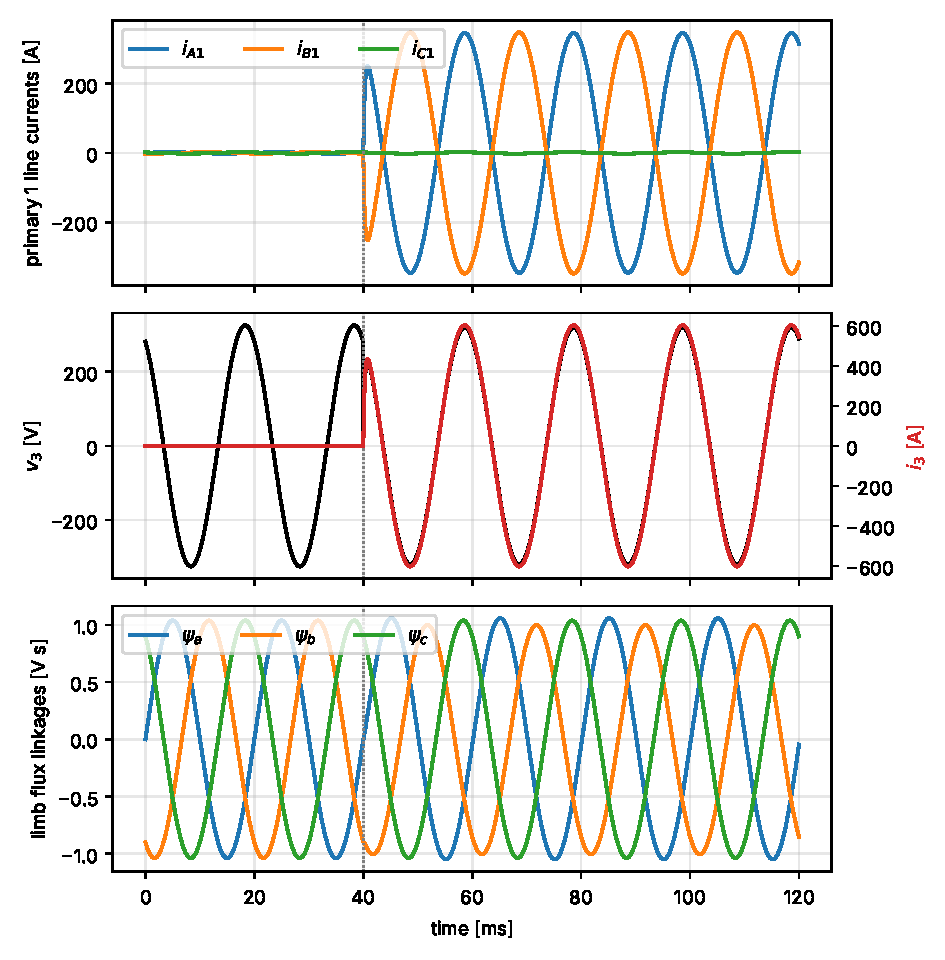
\includegraphics[width=0.68\linewidth]{figures/load_step_rated_load.pdf}
\caption{Time-domain check, default parameters and distribution $\vect{w}=[1,-1,0]$: no load from the steady state, rated resistive load connected at $t = \SI{40}{ms}$ (dotted line). Top: primary-1 line currents, the load current appears in lines $A$ and $B$ only, line $C$ keeps the magnetizing current. Middle: secondary voltage and current. Bottom: flux linkages of the three limbs, balanced before and after the step apart from the resistive and leakage drops.}
\label{fig:step}
\end{figure}

\begin{figure}[htbp]
\centering
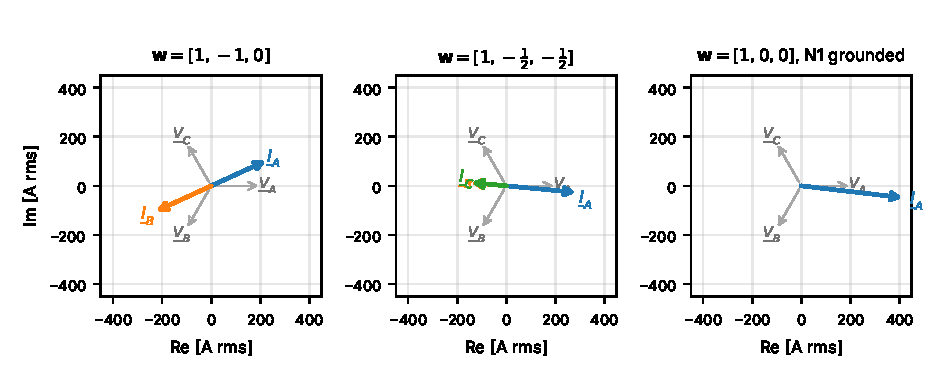
\includegraphics[width=0.95\linewidth]{figures/line_currents_distributions.pdf}
\caption{Primary-1 line currents (rms phasors) at rated resistive load for the three distributions; the grey arrows are the phase voltages. Left: line-to-line arrangement, $\ph{I}_A = -\ph{I}_B$. Centre: T-type arrangement, $\ph{I}_B = \ph{I}_C = -\ph{I}_A/2$ (the two phasors coincide). Right: single-limb arrangement with the neutral grounded, the whole current in line $A$ and in the neutral.}
\label{fig:lines}
\end{figure}

\section{Conclusions and open points}
\label{sec:conclusions}

The transformer with two star primaries and a single-phase secondary is described by a seven-winding model with three magnetizing degrees of freedom, one per limb, and a $3\times3$ magnetizing inductance with a positive-sequence and a zero-sequence value. Under a balanced supply the output is $n_3 g_w V_1/\sqrt3$, with the phase and the gain fixed by the distribution of the secondary turns on the limbs; the single-phase load is reflected on the lines with the same pattern as the turns and always produces a negative-sequence current equal to the positive-sequence one; the short-circuit impedance referred to the secondary is $z_3 + 2z_1$ for every distribution without zero sequence; a distribution with zero sequence needs the neutral, otherwise the load is carried by the zero-sequence flux and the other limbs over-flux; two primaries fed by two sources exchange a circulating current limited only by the two leakage impedances.

Four points depend on the actual unit and should be confirmed on it, or measured, before the model is used quantitatively:
\begin{enumerate}
\item the distribution of the secondary coils on the limbs, i.e. the vector $\vect{w}$ (line-to-line, T type or single limb) and the sign convention of the terminals $s_1$, $s_2$;
\item whether the two primaries are wound on the same core with the same sense (Yy0) or there is a displacement between them, and whether the neutrals are accessible;
\item the short-circuit impedance from the secondary with one primary supplied, and with both in parallel, to set $r_1$, $l_1$, $r_2$, $l_2$, $r_3$, $l_3$;
\item the zero-sequence magnetizing inductance $l_{m0}$ (three-limb core or bank), relevant only if the neutral carries current or the distribution has a zero sequence.
\end{enumerate}

\begin{thebibliography}{9}

\bibitem{fitzgerald}
A.~E.~Fitzgerald, C.~Kingsley~Jr., and S.~D.~Umans,
\emph{Electric Machinery}, 6th ed. New York, NY, USA: McGraw-Hill, 2003.

\bibitem{kulkarni}
S.~V.~Kulkarni and S.~A.~Khaparde,
\emph{Transformer Engineering: Design, Technology, and Diagnostics}, 2nd ed.
Boca Raton, FL, USA: CRC Press, 2013 (zero-sequence behaviour of three-limb cores).

\bibitem{winders}
J.~J.~Winders~Jr.,
\emph{Power Transformer Principles and Applications}.
New York, NY, USA: Marcel Dekker, 2002.

\bibitem{chenguo}
B.-K.~Chen and B.-S.~Guo,
``Three-phase models of specially connected transformers,''
\emph{IEEE Trans. Power Del.}, vol.~11, no.~1, pp.~323--330, Jan. 1996.

\bibitem{scott}
D.~Bagnara, \emph{The Scott-T Transformer: Three-Phase to Two-Phase Conversion and its Simscape Implementation},
pwr-control repositories-documentation, \texttt{research/electrical\_machines/transformers/scott}.

\bibitem{simscape}
The MathWorks, Inc., \emph{Simscape Language Guide}, Natick, MA, USA.

\end{thebibliography}

\end{onehalfspace}
\end{document}
